%%%%%%%% HarnessFlow + MiHaCoBench technical report (ICML 2024 format) %%%%%%%%
\documentclass{article}

\usepackage{microtype}
\usepackage{graphicx}
\usepackage{booktabs}
\usepackage{hyperref}
\usepackage{amsmath}
\usepackage{amssymb}
\usepackage{pifont}
\usepackage{xcolor}
\usepackage{tikz}
\usetikzlibrary{positioning,arrows.meta,fit,backgrounds}
\usepackage{pgfplots}
\pgfplotsset{compat=1.16}

\newcommand{\theHalgorithm}{\arabic{algorithm}}

% Camera-ready style so author block renders (this is a tech report, not a blind submission).
\usepackage[accepted]{icml2024}

\icmltitlerunning{HarnessFlow and MiHaCoBench}

% palette
\definecolor{hfblue}{HTML}{1F4E79}
\definecolor{hfteal}{HTML}{2A7D7B}
\definecolor{hfamber}{HTML}{B5651D}
\definecolor{hfgray}{HTML}{EceEf1}

\begin{document}

\twocolumn[
\icmltitle{HarnessFlow and MiHaCoBench: A Portable Multi-Agent Workflow Pack\\
           for AI Coding Assistants and a Harness-Level Benchmark}

\icmlsetsymbol{equal}{*}

\begin{icmlauthorlist}
\icmlauthor{Hang Yu}{hf}
\end{icmlauthorlist}

\icmlaffiliation{hf}{HarnessFlow Project}
\icmlcorrespondingauthor{Hang Yu}{hangyu8123@gmail.com}

\icmlkeywords{LLM agents, coding agents, agentic workflows, benchmarking, software engineering}

\vskip 0.3in
]

\printAffiliationsAndNotice{}

\begin{abstract}
Modern AI coding assistants are powerful but \emph{one-shot}: given a request they
edit code immediately, with no structured analysis, no self-criticism, no
validation, and no memory across requests. We present \textbf{HarnessFlow}, a
portable Markdown instruction pack---no runtime, no build step---that turns any
compatible assistant (Claude Code, Codex, VS Code + Copilot) into a disciplined
multi-agent system: it classifies each request into one of eight categories,
fans out parallel analysis agents, challenges its own plan, validates with a QA
pass, and records what it learned to persistent repository memory. HarnessFlow
ships every workflow in three modes---\textsc{general} (thorough),
\textsc{fast} (token-efficient), and \textsc{skill} (community-skill-backed)---so
users trade thoroughness against cost explicitly. On two independent benchmarks
the \textsc{fast} mode reaches the same successful outcome as \textsc{general}
while spending only $39$--$50\%$ of the tokens and shipping the leanest
fully-documented code. To measure these effects rigorously we also built
\textbf{MiHaCoBench}, a Python benchmark that scores the \emph{harness} rather
than the model: it holds the model fixed across arms, enforces grader integrity
as its own correctness test, isolates each task to its specification, and targets
the failure frontier where pipelines actually diverge.
\end{abstract}

\section{Why a Harness?}
\label{sec:intro}

The capability of large language models on code has advanced faster than the
\emph{process} wrapped around them. Left to their defaults, today's coding
assistants behave like an over-eager junior engineer: they read the prompt and
start editing, skipping the steps a careful practitioner takes---surveying the
codebase, weighing alternatives, stress-testing assumptions, verifying the result,
and remembering context for next time. The model may be excellent; the
\emph{harness} around it is thin. This gap is increasingly the bottleneck: the
same model produces markedly different outcomes depending on how its work is
structured \citep{yang2024sweagent,jimenez2024swebench}.

\textbf{HarnessFlow} closes this gap as a \emph{drop-in instruction pack}: no
runtime, no \texttt{npm install}, no build step---only Markdown. Copied into a
repository, it gives any compatible assistant a structured workflow for
\emph{every} request: \emph{classify} the prompt, \emph{route} it to a real
multi-step workflow, \emph{analyze} the code from several angles in parallel,
\emph{challenge} the plan, \emph{validate} the implementation, and \emph{record}
the outcome to repository memory so later requests start with real context. The
same pack runs unmodified on three host tools, so a team standardizes its review
discipline once regardless of which assistant each developer prefers.

This report contributes HarnessFlow's architecture and multi-agent pipeline
(\S\ref{sec:arch}); its three workflow modes and the thoroughness--cost trade-off
they expose, including a benchmark where \textsc{fast} matches \textsc{general} at
half the token budget (\S\ref{sec:modes}--\S\ref{sec:benefits}); and MiHaCoBench,
the instrument we built to evaluate harnesses rather than models
(\S\ref{sec:bench}).

\section{HarnessFlow Architecture}
\label{sec:arch}

HarnessFlow is five cooperating pieces of Markdown. (1)~A per-platform
\emph{router} (\texttt{CLAUDE.md}, \texttt{AGENTS.md}, or
\texttt{copilot-instructions.md}) classifies each prompt. (2)~Three
\emph{workflow families} under \texttt{workflow/} hold eight category instruction
files each. (3)~Fifteen \emph{worker subagents} under \texttt{agents/} provide the
roles the workflows orchestrate. (4)~A shared \emph{workflow contract}
(\texttt{\_lib/workflow\_contract.md}) fixes cross-cutting rules. (5)~A
\emph{philosophy} document encodes the behavioral core. Persistent
\emph{repository memory} lives under \texttt{repo\_info/}.

\textbf{Routing.} The router reads the prompt and selects exactly one of eight
categories---\emph{Code}, \emph{Refactor}, \emph{Debug}, \emph{Query},
\emph{Correctness Check}, \emph{Exec}, \emph{PR Creation}, and \emph{Initialize}.
Trigger keywords are soft signals; classification is by primary intent. An
explicit \texttt{mode:} marker (or its absence) selects one of three families.
The router then reads the matching \texttt{<category>.instructions.md} file in
full and follows it step-by-step; multiple intents are handled sequentially.

\textbf{The pipeline.} Figure~\ref{fig:pipeline} shows the \textsc{general}
\emph{Code} workflow, representative of the mutating workflows. The main agent
condenses repository memory into a context digest, then launches three analysts
in parallel---\emph{Focus} (only the most relevant files), \emph{Broad} (the whole
pipeline upstream to downstream), and \emph{Free} (its own judgment). A Senior
Engineer reconciles their plans; the main agent synthesizes a final plan; a
\emph{Devil's Advocate} attacks it for regressions while an \emph{Online
Researcher} checks live sources. After an opt-in approval gate, an Implementer
writes the code, and a parallel Senior + QA pass verifies it before the outcome is
written back to memory. The \emph{Refactor} workflow widens the fan-out to six
specialist analysts reviewed by a Principal Engineer.

\textbf{Cross-cutting guarantees.} The contract enforces \emph{model parity}
(subagents must never downgrade from the orchestrator's model, so quality is not
silently lost in a sub-call), a \emph{two-mode approval gate} (autonomous by
default; opt-in plan-only review triggered by phrases like ``plan only'' or ``no
file changes''), and universal safety rules (never commit to GitHub, never write
spam files, never use \texttt{sudo}). The philosophy document embeds four
guidelines---\emph{Think Before Coding}, \emph{Simplicity First}, \emph{Surgical
Changes}, and \emph{Goal-Driven Execution}---so that, by construction, every
changed line traces to the request.

\begin{figure}[t]
\centering
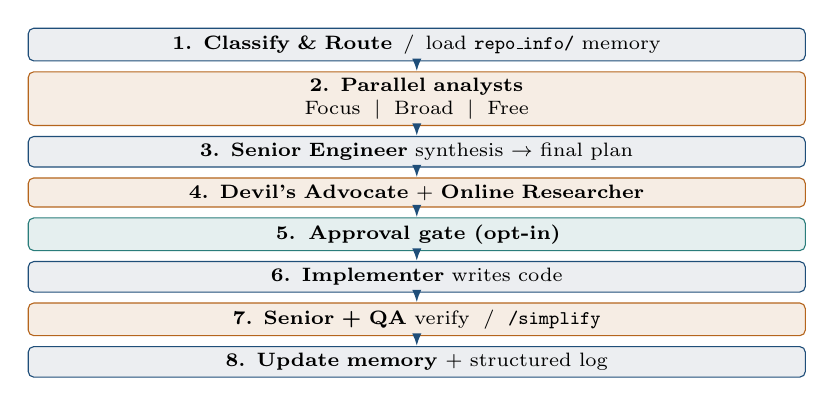
\begin{tikzpicture}[
  node distance=1.25mm and 0mm,
  box/.style={draw=hfblue, fill=hfgray, rounded corners=2pt, align=center,
              text width=0.80\columnwidth, inner sep=2.4pt, font=\scriptsize},
  hot/.style={box, draw=hfamber, fill=hfamber!12},
  gate/.style={box, draw=hfteal, fill=hfteal!12, font=\scriptsize\bfseries},
  arr/.style={-{Latex[length=1.6mm]}, hfblue, thick}
]
\node[box] (route) {\textbf{1. Classify \& Route} \,/\, load \texttt{repo\_info/} memory};
\node[hot, below=of route] (analyst) {\textbf{2. Parallel analysts}\\ Focus \;\textbar\; Broad \;\textbar\; Free};
\node[box, below=of analyst] (senior) {\textbf{3. Senior Engineer} synthesis $\rightarrow$ final plan};
\node[hot, below=of senior] (challenge) {\textbf{4. Devil's Advocate} + \textbf{Online Researcher}};
\node[gate, below=of challenge] (gate) {5. Approval gate (opt-in)};
\node[box, below=of gate] (impl) {\textbf{6. Implementer} writes code};
\node[hot, below=of impl] (qa) {\textbf{7. Senior + QA} verify \;/\; \texttt{/simplify}};
\node[box, below=of qa] (mem) {\textbf{8. Update memory} + structured log};
\foreach \a/\b in {route/analyst, analyst/senior, senior/challenge,
                   challenge/gate, gate/impl, impl/qa, qa/mem}
  \draw[arr] (\a) -- (\b);
\end{tikzpicture}
\caption{The \textsc{general} \emph{Code} pipeline. Amber stages spawn parallel
subagents. \textsc{fast} executes stages 2--3 inline in the main agent and keeps
a single subagent step at stage~4; \textsc{skill} additionally swaps community
skills into planning, implementation, challenge, and review.}
\label{fig:pipeline}
\end{figure}

\section{Three Workflows, One Pack}
\label{sec:modes}

Every category ships in three modes that share the \emph{same} skeleton---read
the contract, gather context, plan, challenge, gate, implement, verify, record---
but differ in how much machinery they spend (Table~\ref{tab:modes}).

\textbf{\textsc{general} (\texttt{mode: general}, the default).} The thorough
variant with the widest fan-out: three to six dedicated planning analysts, a
Senior or Principal Engineer plan review, a Devil's Advocate / Online Researcher
critique pair, and a \emph{separate} Senior + QA verification stage that can run
the full pipeline end-to-end. Use it when correctness and breadth dominate cost.

\textbf{\textsc{fast} (\texttt{mode: fast}).} The token-efficient twin. It folds
the planning analysts and the post-hoc review subagents \emph{into the main
agent}, which does analysis, planning, and implementation inline and spawns
subagents in exactly one step---the Devil's Advocate + Online Researcher
challenge. Verification becomes a structured self-review (``assume every change
is wrong and explain why'') plus native review skills and a single remediation
pass. The instruction files are roughly half the size of their \textsc{general}
counterparts, and---crucially---the empirical outcome is unchanged
(\S\ref{sec:benefits}).

\textbf{\textsc{skill} (\texttt{mode: skill}).} The \textsc{fast} pipeline with
eligible steps---planning, implementation, debugging, challenge, research,
correctness---delegated to confirmed community skills, each verified at
$\geq\!1000$ GitHub stars (e.g.\ \texttt{writing-plans} and
\texttt{systematic-debugging} from a $229{,}665$-star collection) and kept behind
an \emph{inline fallback} so the workflow never blocks if a skill is absent. A
team rides battle-tested external tooling for generic steps while keeping
HarnessFlow's structure, gates, and memory intact.

\begin{table}[t]
\caption{The three workflow modes. ``Subagent spawns'' counts the dedicated
parallel roles a \emph{Code} run launches.}
\label{tab:modes}
\vskip 0.05in
\begin{center}
\begin{small}
\setlength{\tabcolsep}{3.4pt}
\begin{tabular}{lccc}
\toprule
 & \textsc{general} & \textsc{fast} & \textsc{skill}\\
\midrule
Planning analysts      & 3--6        & inline      & inline$^{\dagger}$\\
Subagent spawns (Code) & $\sim$8     & 2           & 2$^{\dagger}$\\
Review stage           & Senior+QA   & self/native & skill/native\\
Approval gate          & opt-in      & opt-in      & opt-in\\
Repo memory            & yes         & yes         & yes\\
Relative token cost    & $1.0\times$ & $0.4$--$0.5\times$ & $\approx$\,fast\\
\bottomrule
\end{tabular}
\end{small}
\end{center}
$^{\dagger}$\,\textsc{skill} mirrors \textsc{fast}'s structure but routes
eligible steps to community skills with inline fallbacks.
\vskip -0.15in
\end{table}

\section{What Users Get}
\label{sec:benefits}

The headline benefit is that \emph{thoroughness becomes a dial, not a gamble}.
We measured the trade-off on two independent benchmarks with the \emph{model held
constant} (Sonnet-class subagents, Opus-class orchestrator) so the comparison
isolates the harness, not the model: a $1{,}000$-line greenfield OpenCV +
scikit-learn build (``ShapeLab''), and a real SWE-bench bug fix
(\texttt{sympy\_\_sympy-24213}). Across both, \textsc{fast} reached the
\emph{same successful outcome} as \textsc{general} while spending only
$39$--$50\%$ of the tokens (Figure~\ref{fig:tokens}) and, on ShapeLab, shipped the
leanest fully-documented code of any arm (Table~\ref{tab:quality}).

\begin{figure}[t]
\centering
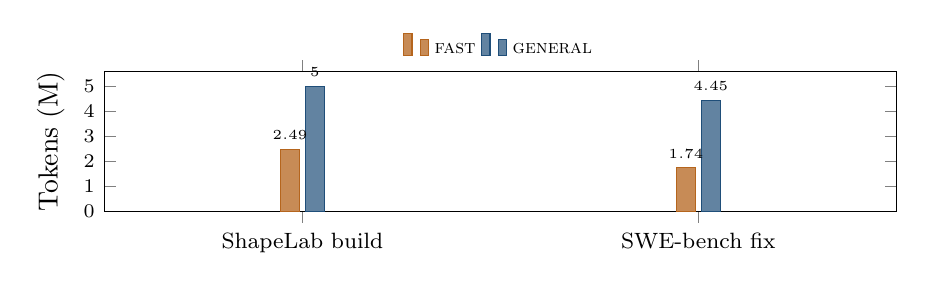
\begin{tikzpicture}
\begin{axis}[
  width=0.96\columnwidth, height=3.35cm,
  ybar, bar width=7pt,
  ymin=0, ymax=5.6,
  ylabel={Tokens (M)}, ylabel near ticks,
  symbolic x coords={ShapeLab build, SWE-bench fix},
  xtick=data, x tick label style={font=\footnotesize},
  ytick={0,1,2,3,4,5}, tick label style={font=\scriptsize},
  legend style={font=\scriptsize, at={(0.5,1.02)}, anchor=south,
                legend columns=2, draw=none},
  enlarge x limits=0.5,
  nodes near coords, every node near coord/.append style={font=\tiny},
]
\addplot[fill=hfamber!75, draw=hfamber] coordinates {(ShapeLab build,2.49) (SWE-bench fix,1.74)};
\addplot[fill=hfblue!70, draw=hfblue] coordinates {(ShapeLab build,5.00) (SWE-bench fix,4.45)};
\legend{\textsc{fast}, \textsc{general}}
\end{axis}
\end{tikzpicture}
\caption{Token cost at \emph{identical} outcomes. \textsc{fast} reaches the same
resolved/verified result as \textsc{general} at $2.0$--$2.6\times$ lower cost.}
\label{fig:tokens}
\end{figure}

\begin{table}[t]
\caption{Quality at equal outcome (ShapeLab build; SWE-bench fix verified). The
baseline is the same model with no harness.}
\label{tab:quality}
\vskip 0.05in
\begin{center}
\begin{small}
\begin{tabular}{lccc}
\toprule
Metric & baseline & \textsc{fast} & \textsc{general}\\
\midrule
Code lines (AST)        & 1{,}225 & \textbf{860} & 1{,}173\\
Docstring coverage      & 96.3\%  & \textbf{100\%} & 100\%\\
Contract tests passed   & 7/10    & \textbf{10/10} & 10/10\\
Self-verified pre-ship  & none    & \textbf{32 green} & yes\\
SWE canonical fix       & \ding{55} & \checkmark & \checkmark\\
\bottomrule
\end{tabular}
\end{small}
\end{center}
\vskip -0.15in
\end{table}

Beyond cost, the pack pays off in three ways. \emph{Portability:} one
instruction pack standardizes review discipline across Claude Code, Codex, and
Copilot. \emph{Quality under self-criticism:} the no-harness baseline produced a
non-canonical, unverified SWE-bench patch and passed only $7/10$ contract tests,
whereas both harnessed modes produced the exact canonical fix, verified, at
$10/10$. \emph{Memory and safety:} outcomes persist to \texttt{repo\_info/} so the
next request starts informed, while opt-in plan review and hard prohibitions on
commits, spam files, and \texttt{sudo} keep autonomy bounded.

\section{MiHaCoBench: Scoring the Harness}
\label{sec:bench}

Building HarnessFlow surfaced a measurement problem: standard code benchmarks
\citep{chen2021codex,austin2021mbpp,jain2024livecodebench} score a \emph{model}
in isolation, but a harness contributes prompt handling, multi-step planning,
tool use, and long-horizon consistency that those benchmarks never exercise. We
therefore built \textbf{MiHaCoBench}, both the development test bench for
HarnessFlow and a standalone instrument for evaluating \emph{any} coding pipeline.
Its design draws on SWE-bench, BigCodeBench, and LiveCodeBench
\citep{jimenez2024swebench,zhuo2024bigcodebench,jain2024livecodebench}. Four
properties distinguish it.

\textbf{1. It scores the harness, not the model.} Every arm---no-harness
baseline, \textsc{fast}, \textsc{skill}, \textsc{general}---runs the same tasks at
the \emph{same} model with verified parity, so a score delta is attributable to
\emph{process}, not capability.

\textbf{2. Grader integrity is its own test.} Borrowing SWE-bench's
\textsc{fail\_to\_pass} / \textsc{pass\_to\_pass} discipline, each task ships a
hidden \emph{gold} reference the grader must accept and a deliberately
\emph{broken} reference it must reject. The default \texttt{--self-check} mode
proves all $69$ graders valid (gold passes, broken fails) \emph{before} any
candidate is scored; graders test only the public contract, so a harness cannot
be rewarded for matching an internal layout.

\textbf{3. Spec-only isolation and contamination control.} The scaffolder copies
\emph{only} each task's \texttt{TASK.md} (plus committed inputs) into an external
workspace and refuses any target inside the repository, so an agent never sees
graders, references, or sibling tasks. Reproducibility is pinned: Python 3.11.5,
committed datasets, fixed seeds, \texttt{PYTHONHASHSEED=0}. Contamination is
resisted with domain-specific entry-point names, twisted classics, and a dated
\texttt{TASK.md} per task for temporal filtering.

\textbf{4. A failure-frontier task design.} The suite is $69$ tasks across ten
\emph{weighted} categories (easy$=1$ up to competitive$=8$), so a harness cannot
inflate its score by acing only the easy ones. Crucially, MiHaCoBench
\emph{discovered} that well-specified tasks under-discriminate: a careful frontier
model reads the spec and one-shots them, and the arms tie. The suite therefore
targets the regime where single shots fail---hard complexity gates that physically
time out wrong-complexity solutions, multi-file fault localization, statistical
surface-form twists where the memorized answer is wrong, and long state cascades.
This finding is itself the contribution: \emph{separating harnesses requires
failure-frontier tasks, not merely well-specified ones.}

\textbf{What we observe.} Exploratory single-run ($n{=}1$) comparisons on a
$79$-task superset bear this out: the arms tie on the large majority of tasks
($72/79$), and the few that discriminate---e.g.\ a boundary-ambiguity pagination
task that splits the no-harness baseline from the harnessed arms---are exactly the
failure-frontier items the design targets. We report these as directional, not
statistically significant; their value is in showing that the \emph{instrument}
localizes where harnesses diverge---precisely what a development test bench must
do.

\section{Conclusion}

Much of the value left on the table by AI coding assistants is recoverable with
\emph{process}, not a bigger model. HarnessFlow turns a one-shot tool into a
disciplined collaborator---classify, analyze in parallel, self-challenge,
validate, remember---with three modes that price thoroughness explicitly
(\textsc{fast} matching \textsc{general} at half the cost). MiHaCoBench makes the
claim testable by scoring the pipeline, not the model, on the failure frontier
where pipelines diverge. Build the harness; measure the harness.

\bibliography{references}
\bibliographystyle{icml2024}

\end{document}
